En la sección pasada vimos cómo se puede usar PPA para demostrar teoremas. Pero,
¿cómo funciona por detrás? ¿Como asegura la validez lógica de las
demostraciones escritas por el usuario?

\section{Certificados}

Los programas de PPA se \textbf{certifican}, generando una demostración en
deducción natural. ¿Por qué? El lenguaje de PPA es complejo, la implementación
no es trivial. Si se escribe una demostración, para confiar en que es correcta
hay que confiar en la implementación de PPA.

Pero si PPA genera una demostración de bajo nivel, que usa las reglas de un
sistema lógico simple como deducción natural, entonces cualquiera que desconfíe
podría fácilmente escribir un chequeador, o usar uno confiable. Por eso genera
demostraciones en deducción natural, haciendo que cumpla con el \textbf{criterio
de de Bruijn}

\begin{definition}{Criterio de de Bruijn \cite{freek-bruijn}.} Un asistente de
    demostración que satisface que sus demostraciones puedan ser chequeadas por
    un programa independiente, pequeño y confiable se dice que cumple con el
    criterio de de Bruijn.
\end{definition}

El módulo de PPA que \textit{certifica} las demostraciones de alto nivel de PPA
generando una demostración en deducción natural es el \modCertifier{}. Si
bien toda demostración que genere debería ser correcta, para atajar posibles
errores siempre se chequean con el \modChecker{} de DN.


\duda{Para pablo: pero si emite certificados que no corresponden a la demo original y chequean siempre, por ej. siempre el mismo, no estaría mal igual? Tenés que confiar también en la parte que emite el certificado.}

\section{Certificador}

El \modCertifier en realidad no genera una sola demostración de deducción
natural, sino que al poder haber más de un teorema en un archivo PPA, este
genera un \textbf{contexto} compuesto por una lista ordenada de
\textbf{hipótesis}. Hay dos tipos de hipótesis

\begin{itemize}
    \item Teoremas: Son fórmulas con demostraciones asociadas.
    \item Axiomas: Son fórmulas que se asumen válidas (pueden ser usadas para
    modelar una teoría)
\end{itemize}

\begin{figure}[H]
    \centering
    \begin{multicols}{2}
        \begin{tabular}{c}
            \lstinputlisting{listings/certifier/two-theorems.ppa}
        \end{tabular}
        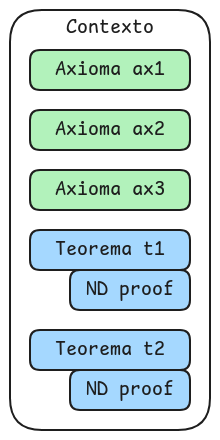
\includegraphics[scale=0.5]{img/ppa-context.png}
    \end{multicols}
    \caption{Contexto resultante de certificar de un programa}
\end{figure}


Por lo tanto, en vez de chequear demostraciones, se chequean contextos: Una
demostración será válida en el \textit{prefijo estricto del contexto} que la
contiene. Es decir, a la hora de chequearla, se deben asumir como ciertas todas
las hipótesis que fueron definidas previamente.

Cada demostración de un teorema tendrá además un \textit{contexto local}. Las
afirmaciones auxiliares que no afectan la tesis (\lstinline{have},
\lstinline{claim}, \lstinline{consider}, etc.) se agregan como teoremas. Por lo
tanto, cuando se citen, se pegan sus demostraciones. Por otro lado, algunos
comandos agregan axiomas, los mismos que en deducción natural agregan fórmulas
al contexto (\lstinline{suppose} y \lstinline{consider}). Es correcto asumir
como ciertas esas hipótesis, porque lo mismo se hará durante el chequeo de la
demostración en deducción natural.

\begin{figure}[H]
    \centering
    \begin{multicols}{2}
        \begin{tabular}{c}
            \lstinputlisting{listings/certifier/local-context.ppa}
        \end{tabular}
        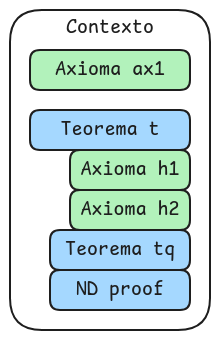
\includegraphics[scale=0.5]{img/ppa-local-context.png}
    \end{multicols}
    \caption{Contexto local}
\end{figure}

\section{Implementación de By}

El \lstinline{by} es el mecanismo principal de demostración en PPA. Genera
automáticamente una demostración de que una fórmula es consecuencia de una lista
de hipótesis. Supongamos que queremos demostrar \lstinline{thus A by h1, ..., hn} y que en el contexto tenemos que las hipótesis $h_i$
corresponden a fórmulas $\formTwo_i$, con $i \in \{1, ..., n\}$. La estrategia es la siguiente

\begin{itemize}
    \item Queremos generar una demostración para la implicación
    \[
        \formTwo_1 \fAnd \formTwo_2 \fAnd \formTwo_3 \fImp \form
    \]
    \item Demostramos por el absurdo: a partir de la negación encontramos una contradicción
    \[
        \formTwo_1 \fAnd \formTwo_2 \fAnd \formTwo_3 \fImp \form
    \]
\end{itemize}

\subsection{Razonamiento por el absurdo}

\todo{DnegElim como regla admisible, y cómo permite razonar por el absurdo}

\subsection{Juntando demostraciones}

\todo{Cut como regla admisible}

\subsection{Unificación}
\label{ppa:sec:unification}

\section{Comandos correspondientes a reglas de inferencia}

Como se puede apreciar en \fullref{ppa:tab:inference-rules-to-commands}, la
mayoría de los comandos se corresponden directamente con reglas de inferencia,
por lo que su traducción es más sencilla.

\section{Comandos adicionales}


